%% V1.0
%% by Gabriel Garcia, gabrcg@gmail.com
%% This is a template for Udacity projects using IEEEtran.cls

%% Be Udacious!

\documentclass[10pt,journal,compsoc]{IEEEtran}

\usepackage[pdftex]{graphicx}    
\hyphenation{op-tical net-works semi-conduc-tor}


\begin{document}

\title{Practicing with the DIGITS Workflow}

\author{Jeremy Hale}

\markboth{Inference project, Robotic Nanodegree, Udacity}%
{}
\IEEEtitleabstractindextext{%

\begin{abstract}
Practicing with the DIGITS Workflow using the conveyor belt dataset from Udacity.
\end{abstract}

% Note that keywords are not normally used for peerreview papers.
\begin{IEEEkeywords}
Robot, IEEEtran, Udacity, \LaTeX, deep learning.
\end{IEEEkeywords}}


\maketitle
\IEEEdisplaynontitleabstractindextext
\IEEEpeerreviewmaketitle
\section{Introduction}
\label{sec:introduction}

\IEEEPARstart{P}{art} of the inference project is practicing simple deep learning networks using the nVidia DIGITS application.

\section{Background / Formulation}
The GoogleLeNet model was chosen. It is a standard model available in the DIGITS application. The model was chosen because the inference time is less than 10 ms and the accuracy is higher than AlexNet. To avoid overfitting, the training was terminated after 5 epochs.

\section{Results}
The requirements for the project were less than 10 milliseconds inference time and greater than 75 percent accuracy. The output of the "evaluate" command is shown below. The accuracy is 75.4 percent and the inference time is less than 6 milliseconds.

\begin{figure}[thpb]
      \centering
      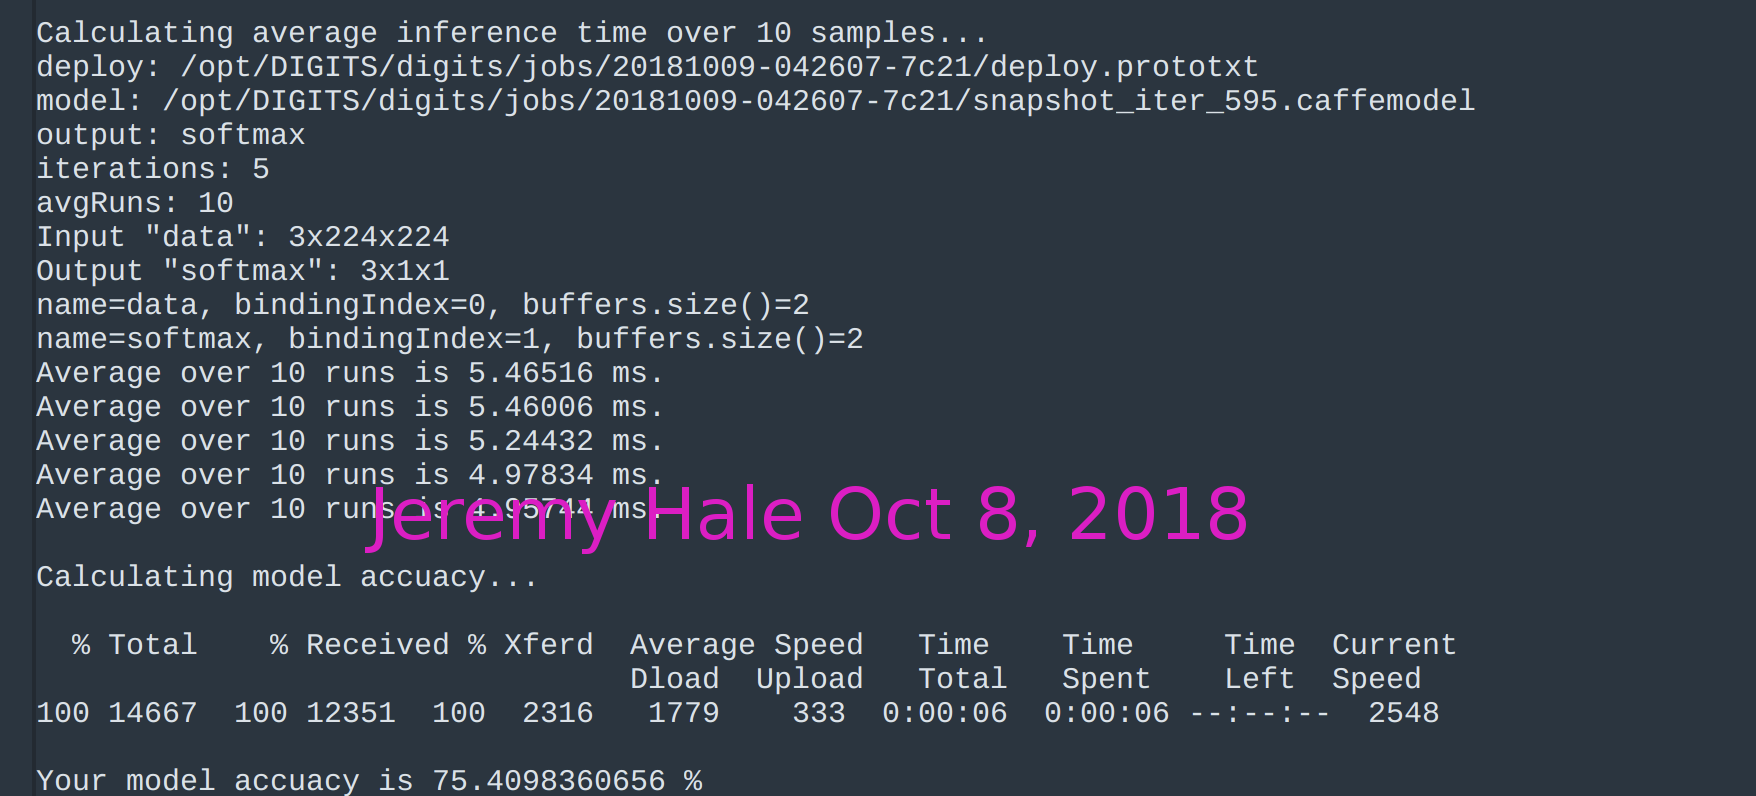
\includegraphics[width=\linewidth]{googlenet_epoch5_water}
      \caption{GoogleLeNet.}
      \label{fig:GoogleLeNet}
\end{figure}

The training plot is shown below.

\begin{figure}[thpb]
      \centering
      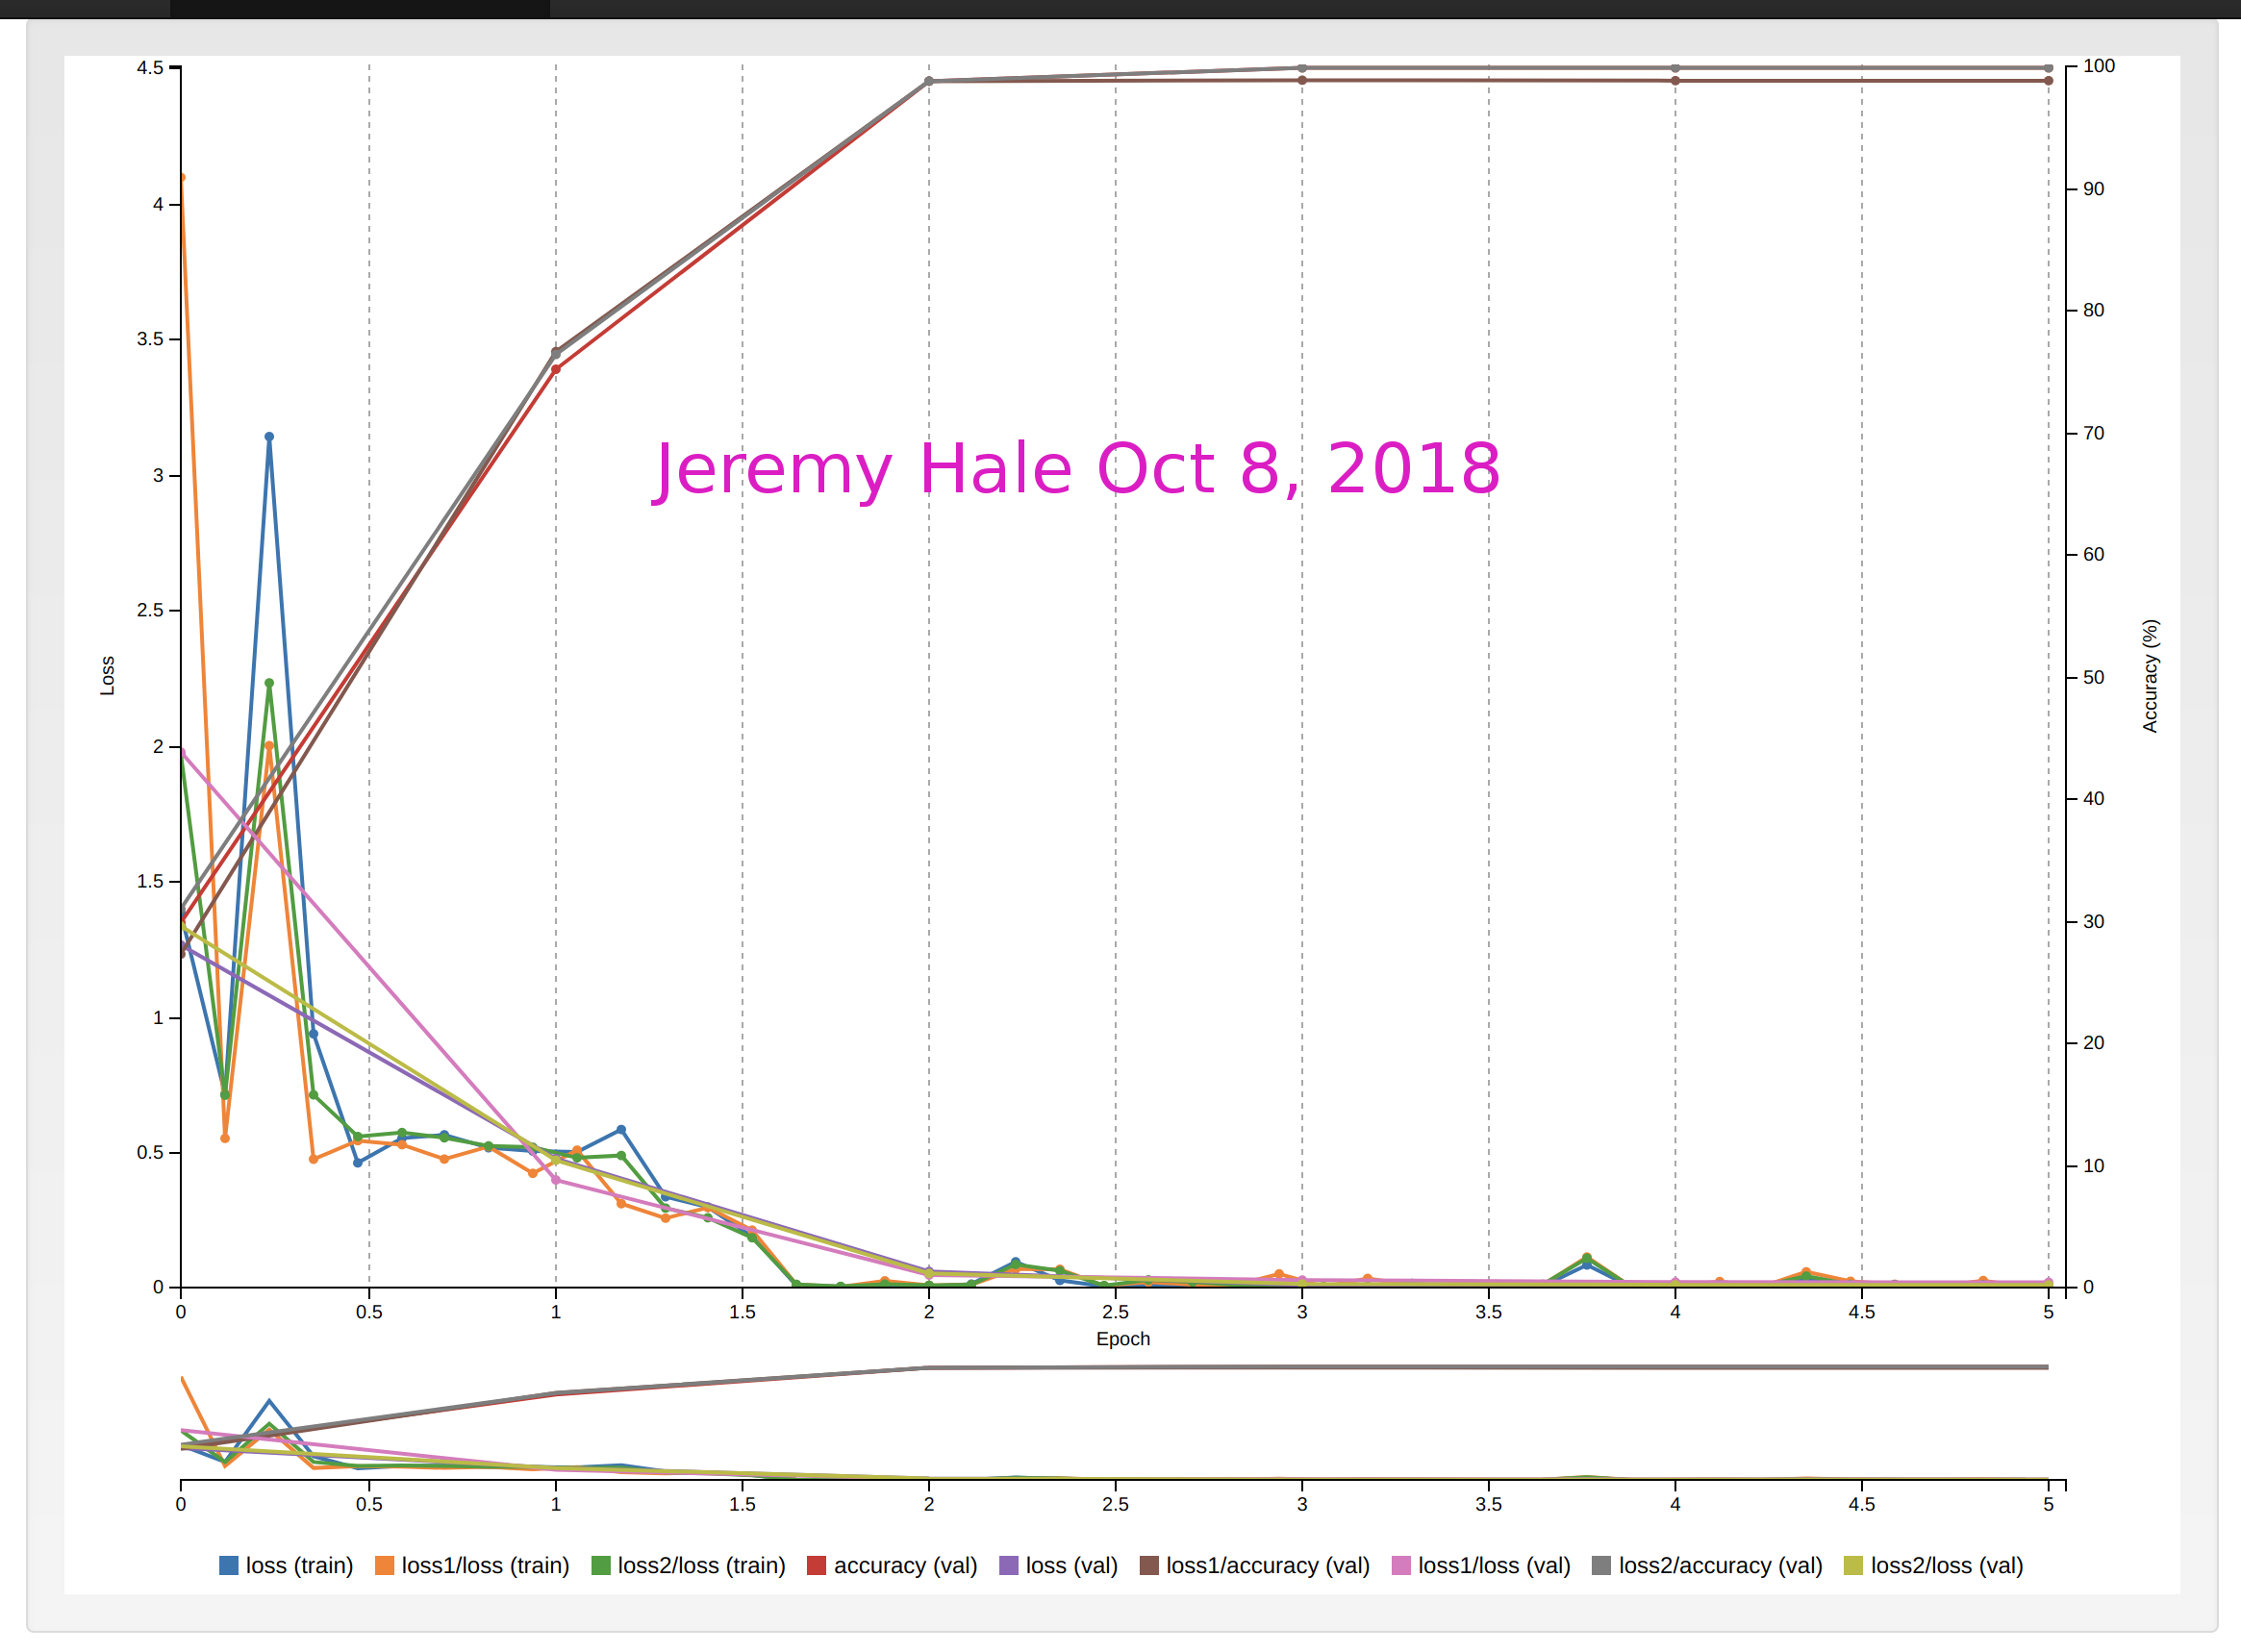
\includegraphics[width=\linewidth]{training_water}
      \caption{Training.}
      \label{fig:training}
\end{figure}

\section{Discussion}

The performance is sufficient for the project requirements. The first attempt trained for 30 epochs; however, this resulted in overfitting and the accuracy of the test data dropped to ~70 percent.

\section{Conclusion / Future work}
The GoogleLeNet model has a reasonable balance of inference time and performance. The saved model is stored in the folder "model\_epoch5". Future work could use a GoogleLeNet model pretrained on ImageNet for higher accuracy.
\bibliography{bib}
\bibliographystyle{ieeetr}

\end{document}